\begin{frame}{VisAQ - Visualizing Air Quality}
    Ziel ist die Entwicklung einer Anwenderorientierte Nutzerschnittstelle für Luftqualitätsdaten
\end{frame}
\begin{frame}{Nutzerstudie}
    Ermittelt Nutzerverhalten und Bedürfnisse
\end{frame}
\begin{frame}{Nutzerstudie - Altersverteilung}
    \begin{figure}[h]
        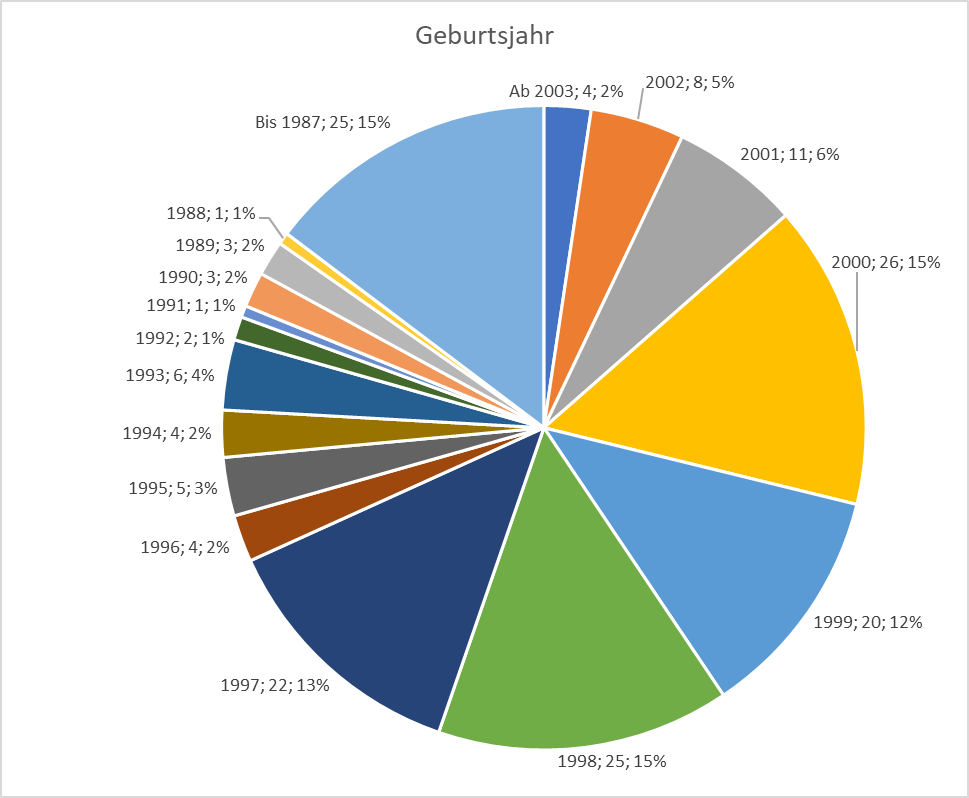
\includegraphics[height=0.7\textheight]{../../media/diagram/geburtsjahr}
    \end{figure}
\end{frame}
\begin{frame}{Nutzerstudie - Selbsteinschätzung}
    \begin{figure}[h]
        \begin{subfigure}[c]{0.49\textwidth}
            \centering        
            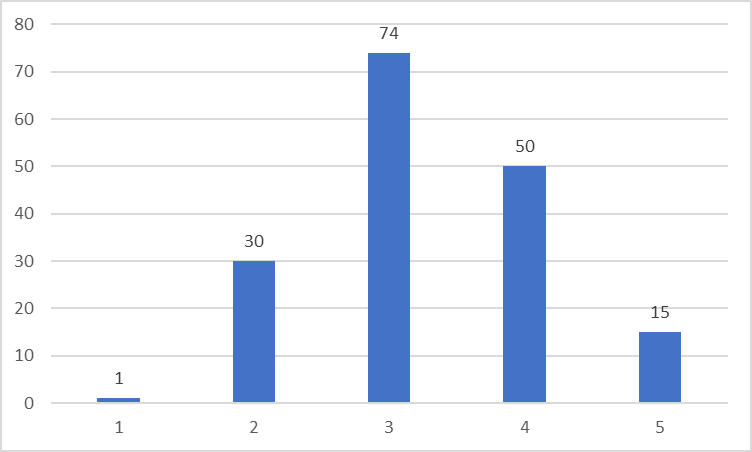
\includegraphics[scale=0.2]{../../media/diagram/eigenesWissen.png}
            \subcaption{Einschätzung zum eigenen Wissen über Luftverschmutzung}
        \end{subfigure}
        \begin{subfigure}[c]{0.49\textwidth}
            \centering        
            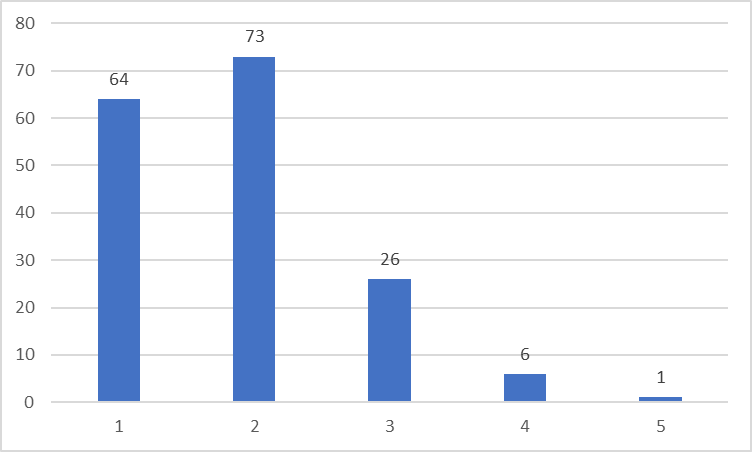
\includegraphics[scale=0.2]{../../media/diagram/WichtigkeitVonInfos.png}
            \subcaption{Einschätzung zur Wichtigkeit von Informationen über Luftverschmutzung}
        \end{subfigure}
    \end{figure}
\end{frame}
\begin{frame}{Nutzerstudie - Aufrufshäufigkeit}
    \begin{figure}[h]
        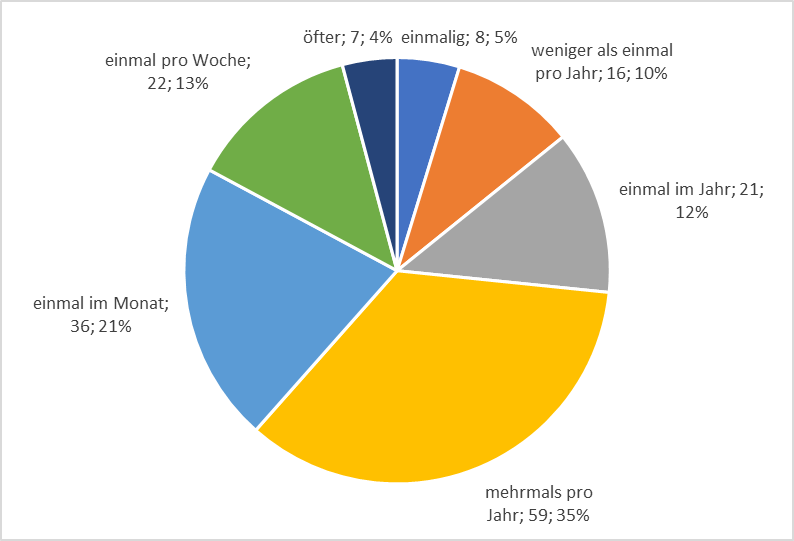
\includegraphics[height=0.7\textheight]{../../media/diagram/aufrufe}
    \end{figure}
\end{frame}
\begin{frame}{Nutzerstudie - Informationsbedürfniss}
    \begin{figure}[h]
        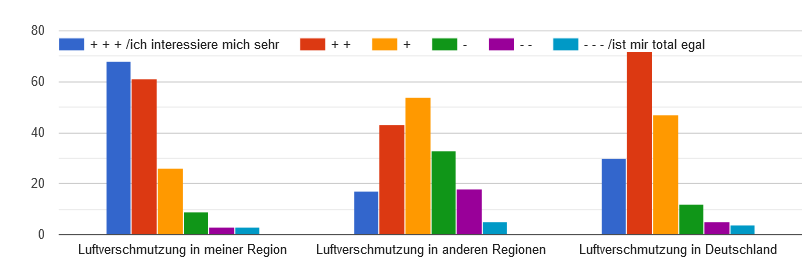
\includegraphics[height=0.35\textheight]{../../media/diagram/interesse}
    \end{figure}
    \begin{figure}[h]
        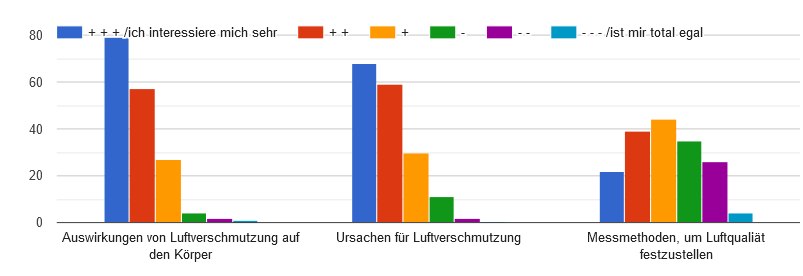
\includegraphics[height=0.35\textheight]{../../media/diagram/interesse2}
    \end{figure}
\end{frame}
\begin{frame}{Nutzerstudie - Sonstige Ergebnisse}
    \centering
    Nutzergeräte
    \\
    \vspace{1cm}
    Allgemeine Anregungen
\end{frame}
\begin{frame}{Abgrenzung}
    \begin{itemize}
        \item Reine Webapplikation
        \item Kein User Management
        \item Nur zum Sensorthings Standart kompatibel
    \end{itemize}
\end{frame}
\begin{frame}{Anforderungen an Hard- und Software}
    \textbf{Server:}\\
    Hardware
    \begin{itemize}
        \item Netzwerkfähige Sensorthings-Datenbank
        \item Webserver
    \end{itemize}
    \pause
    \textbf{Client:}\\
    Hardware
    \begin{itemize}
        \item Eingabegerät zur Interaktion
        \item Netzwerkfähige
        \item Standard-Hardware
    \end{itemize}
    \pause
    Software
    \begin{itemize}
        \item Standard-Betriebsystem
        \item Standard-Browser
    \end{itemize}
\end{frame}